\documentclass{beamer}
\usepackage{ArmenianSlides}

\begin{document}

\title[Memento]{Նախագծման Ձևանմուշներ։ Memento}
\author[Հրաչյա Թանդիլյան\copyright]{Հրաչյա Թանդիլյան}
\date{2020}

%-------------------------------------------------------------------------------------------------
\begin{frame}
\titlepage
\end{frame}
%-------------------------------------------------------------------------------------------------

\section{Նպատակը}
%-------------------------------------------------------------------------------------------------
\begin{frame}\frametitle{Memento}
\begin{block}{Նպատակը}
    Առանց ինկապսուլացիան խախտելու ֆիքսել և պահպանել օբյեկտի ներքին վիճակն այնպես,
    որ օբյեկտը հետագայում հնարավոր լինի բերել այդ վիճակի:
\end{block}
\vfill
Նաև հայտնի է որպես
\begin{itemize}
    \item Token
\end{itemize}
\end{frame}
%-------------------------------------------------------------------------------------------------

\subsection{Մոտիվացիան}
%-------------------------------------------------------------------------------------------------
\begin{frame}\frametitle{Մոտիվացիան}
\begin{center}
    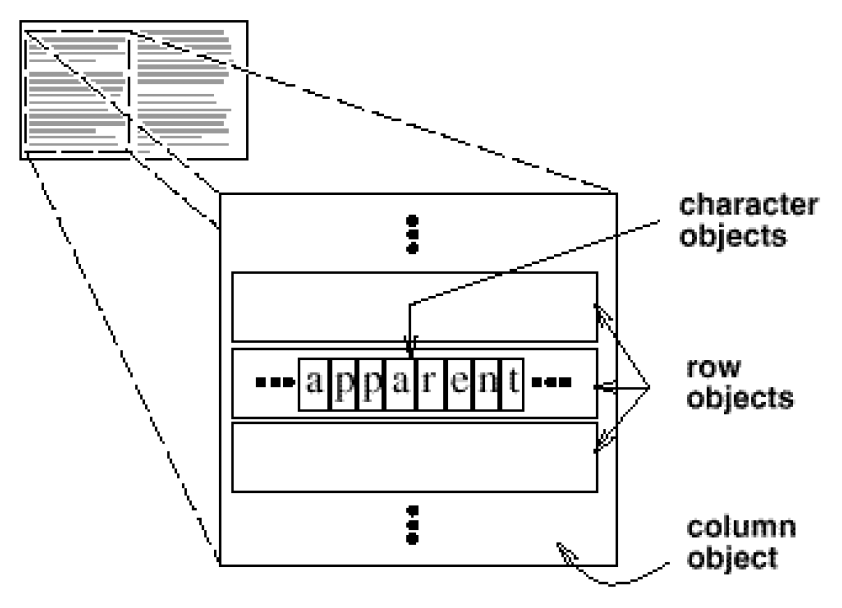
\includegraphics[scale=0.4]{motivation1.png}
    \vfill
    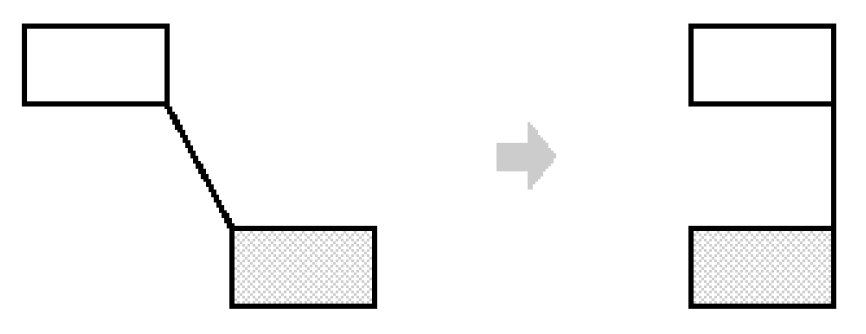
\includegraphics[scale=0.4]{motivation2.png}
\end{center}
\end{frame}
%-------------------------------------------------------------------------------------------------

\subsection{Կիրառելիությունը}
%-------------------------------------------------------------------------------------------------
\begin{frame}\frametitle{Կիրառելիությունը}
Այս Ն.Ձ. պետք է օգտագործել երբ.
\vfill
\begin{enumerate}
    \item Անհրաժեշտ է պահպանել օբյեկտի ֆիքսված պահի ներքին վիճակն այնպես,
    որ օբյեկտը հետագայում հնարավոր լինի վերադարձնել այդ վիճակի: \vfill
    \item Օբյեկտի ներքին վիճակը վերադարձնող անմիջական ինտերֆեյսի տրամադրումը
    կբերի նրա ինկապսուլացիաի խախտման:
\end{enumerate}
\end{frame}
%-------------------------------------------------------------------------------------------------

\section{Կառուցվածքը}
%-------------------------------------------------------------------------------------------------
\begin{frame}\frametitle{Կառուցվածքը}
\begin{center}
    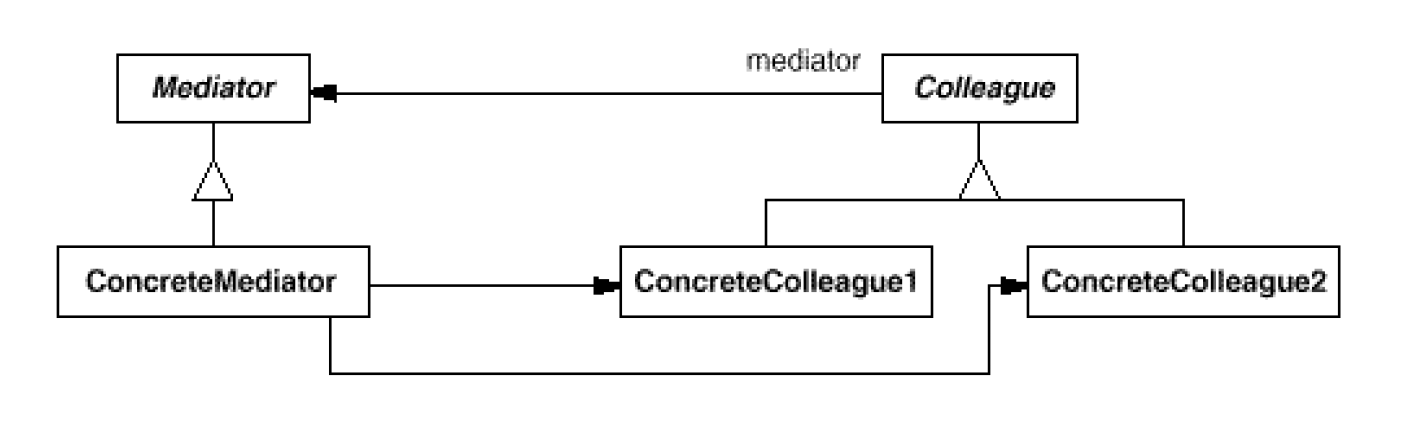
\includegraphics[scale=0.4]{structure1.png}
\end{center}
\end{frame}
%-------------------------------------------------------------------------------------------------

%-------------------------------------------------------------------------------------------------
\begin{frame}\frametitle{Կառուցվածքը}
\begin{center}
    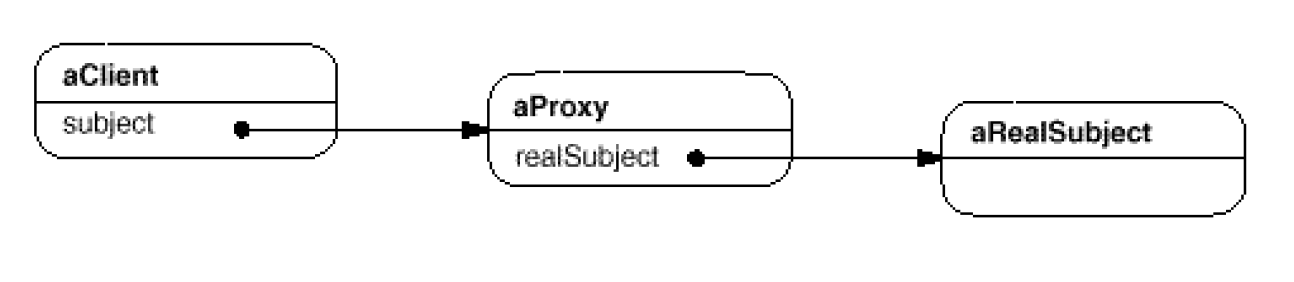
\includegraphics[scale=0.4]{structure2.png}
\end{center}
\end{frame}
%-------------------------------------------------------------------------------------------------

\subsection{Հետևանքները}
%-------------------------------------------------------------------------------------------------
\begin{frame}\frametitle{Հետևանքները}
Այս Ն.Ձ. ունի հետևյալ առավելություններն ու թերությունները.
\vfill
\begin{enumerate}
    \item Ինկապսուլացիաի պահպանում: \vfill
    \item Originator դասի պարզեցում: \vfill
    \item Memento-ի կիրառումը կարող է\\ ծախսատար լինել: \vfill
    \item Լայն և նեղ ինտերֆեյսների սահմանումը:
\end{enumerate}
\end{frame}
%-------------------------------------------------------------------------------------------------

\section{Իրականացումը}
%-------------------------------------------------------------------------------------------------
\begin{frame}\frametitle{Իրականացումը}
\begin{enumerate}
    \item Լեզվային ապահովում: \vfill
    \item Հաջորդական (incremental) փոփոխությունների պահպանում:
\end{enumerate}
\end{frame}
%-------------------------------------------------------------------------------------------------
%-------------------------------------------------------------------------------------------------
\begin{frame}[fragile]\frametitle{Իրականացումը: Լեզվային ապահովում}
\begin{english}
\begin{minted}{cpp}
class State;

class Originator {

public:
    Memento* CreateMemento();
    void SetMemento(const Memento*);

private:
    State* state;

    // Internal data structures
};
\end{minted}
\end{english}
\end{frame}
%-------------------------------------------------------------------------------------------------

%-------------------------------------------------------------------------------------------------
\begin{frame}[fragile]\frametitle{Իրականացումը: Լեզվային ապահովում}
\begin{english}
\begin{minted}{cpp}
class Memento {

public:
    // Narrow public interface
    virtual ~Memento();

private:
    // Wide private interface
    friend class Originator;

    Memento();
    void SetState(State*);
    State* GetState();

private:
    State* state;
};
\end{minted}
\end{english}
\end{frame}
%-------------------------------------------------------------------------------------------------

\subsection{Օրինակ}
%-------------------------------------------------------------------------------------------------
\begin{frame}[fragile]\frametitle{Օրինակ}
\begin{english}
\begin{minted}{cpp}
// Base class for graphical objects in the graphical editor
class Graphic;

class MoveCommand {

public:
    MoveCommand(Graphic* t, const Point& d);
    void Execute();
    void Unexecute();

private:
    ConstraintSolverMemento* state;
    Point delta;
    Graphic* target;
};
\end{minted}
\end{english}
\end{frame}
%-------------------------------------------------------------------------------------------------

%-------------------------------------------------------------------------------------------------
\begin{frame}[fragile]\frametitle{Օրինակ}
\begin{english}
\begin{minted}[fontsize=\scriptsize]{cpp}
class ConstraintSolver {

public:
    static ConstraintSolver* Instance();
    void Solve();

    void AddConstraint(Graphic* startConnection,
                       Graphic* endConnection);

    void RemoveConstraint(Graphic* startConnection,
                          Graphic* endConnection);

    ConstraintSolverMemento* CreateMemento();
    void SetMemento(ConstraintSolverMemento*);

private:
    // Nontrivial state and operations for
    // enforcing connectivity semantics
};
\end{minted}
\end{english}
\end{frame}
%-------------------------------------------------------------------------------------------------

%-------------------------------------------------------------------------------------------------
\begin{frame}[fragile]\frametitle{Օրինակ}
\begin{english}
\begin{minted}{cpp}
class ConstraintSolverMemento {

public:
    virtual ~ConstraintSolverMemento();

private:
    friend class ConstraintSolver;

    ConstraintSolverMemento();

    // Private constraint solver state
};
\end{minted}
\end{english}
\end{frame}
%-------------------------------------------------------------------------------------------------

%-------------------------------------------------------------------------------------------------
\begin{frame}[fragile]\frametitle{Օրինակ}
\begin{english}
\begin{minted}{cpp}
void MoveCommand::Execute () {

    ConstraintSolver* solver = ConstraintSolver::Instance();

    state = solver->CreateMemento(); // Create a memento
    target->Move(delta);
    solver->Solve();
}

void MoveCommand::Unexecute () {

    ConstraintSolver* solver = ConstraintSolver::Instance();

    target->Move(-delta);
    solver->SetMemento(state); // Restore solver state
    solver->Solve();
}
\end{minted}
\end{english}
\end{frame}
%-------------------------------------------------------------------------------------------------

%-------------------------------------------------------------------------------------------------
\begin{frame}[fragile]\frametitle{Օրինակ 2}
\begin{english}
\begin{minted}{cpp}
template <class Item>
class Collection {

public:
    Collection();
    IterationState* CreateInitialState();

    void Next(IterationState&);
    bool IsDone(const IterationState&) const;
    Item CurrentItem(const IterationState&) const;
    IterationState* Copy(const IterationState&) const;

    void Append(const Item&);
    void Remove(const Item&);
};
\end{minted}
\end{english}
\end{frame}
%-------------------------------------------------------------------------------------------------

%-------------------------------------------------------------------------------------------------
\begin{frame}[fragile]\frametitle{Օրինակ 2}
\begin{english}
\begin{minted}{cpp}
class ItemType {

public:
    void process();
    // Other methods
};

Collection<ItemType> c;

std::auto_ptr<IterationState> state(c.CreateInitialState());

while (!c.IsDone(*state)) {

    c.CurrentItem(*state).process();
    c.Next(*state);
}
\end{minted}
\end{english}
\end{frame}
%-------------------------------------------------------------------------------------------------

\section{Առնչվող Ձևանմուշները}
%-------------------------------------------------------------------------------------------------
\begin{frame}\frametitle{Առնչվող Նախագծման Ձևանմուշները}
\begin{itemize}
    \item Command \vfill
    \item Iterator
\end{itemize}
\end{frame}
%-------------------------------------------------------------------------------------------------

\end{document}
